\section{Null tests, negative controls, and failure cases}
\label{app:more_tccon_test}




\subsection{Null tests}
\label{app:null-test}


\begin{figure}[t]
\centering
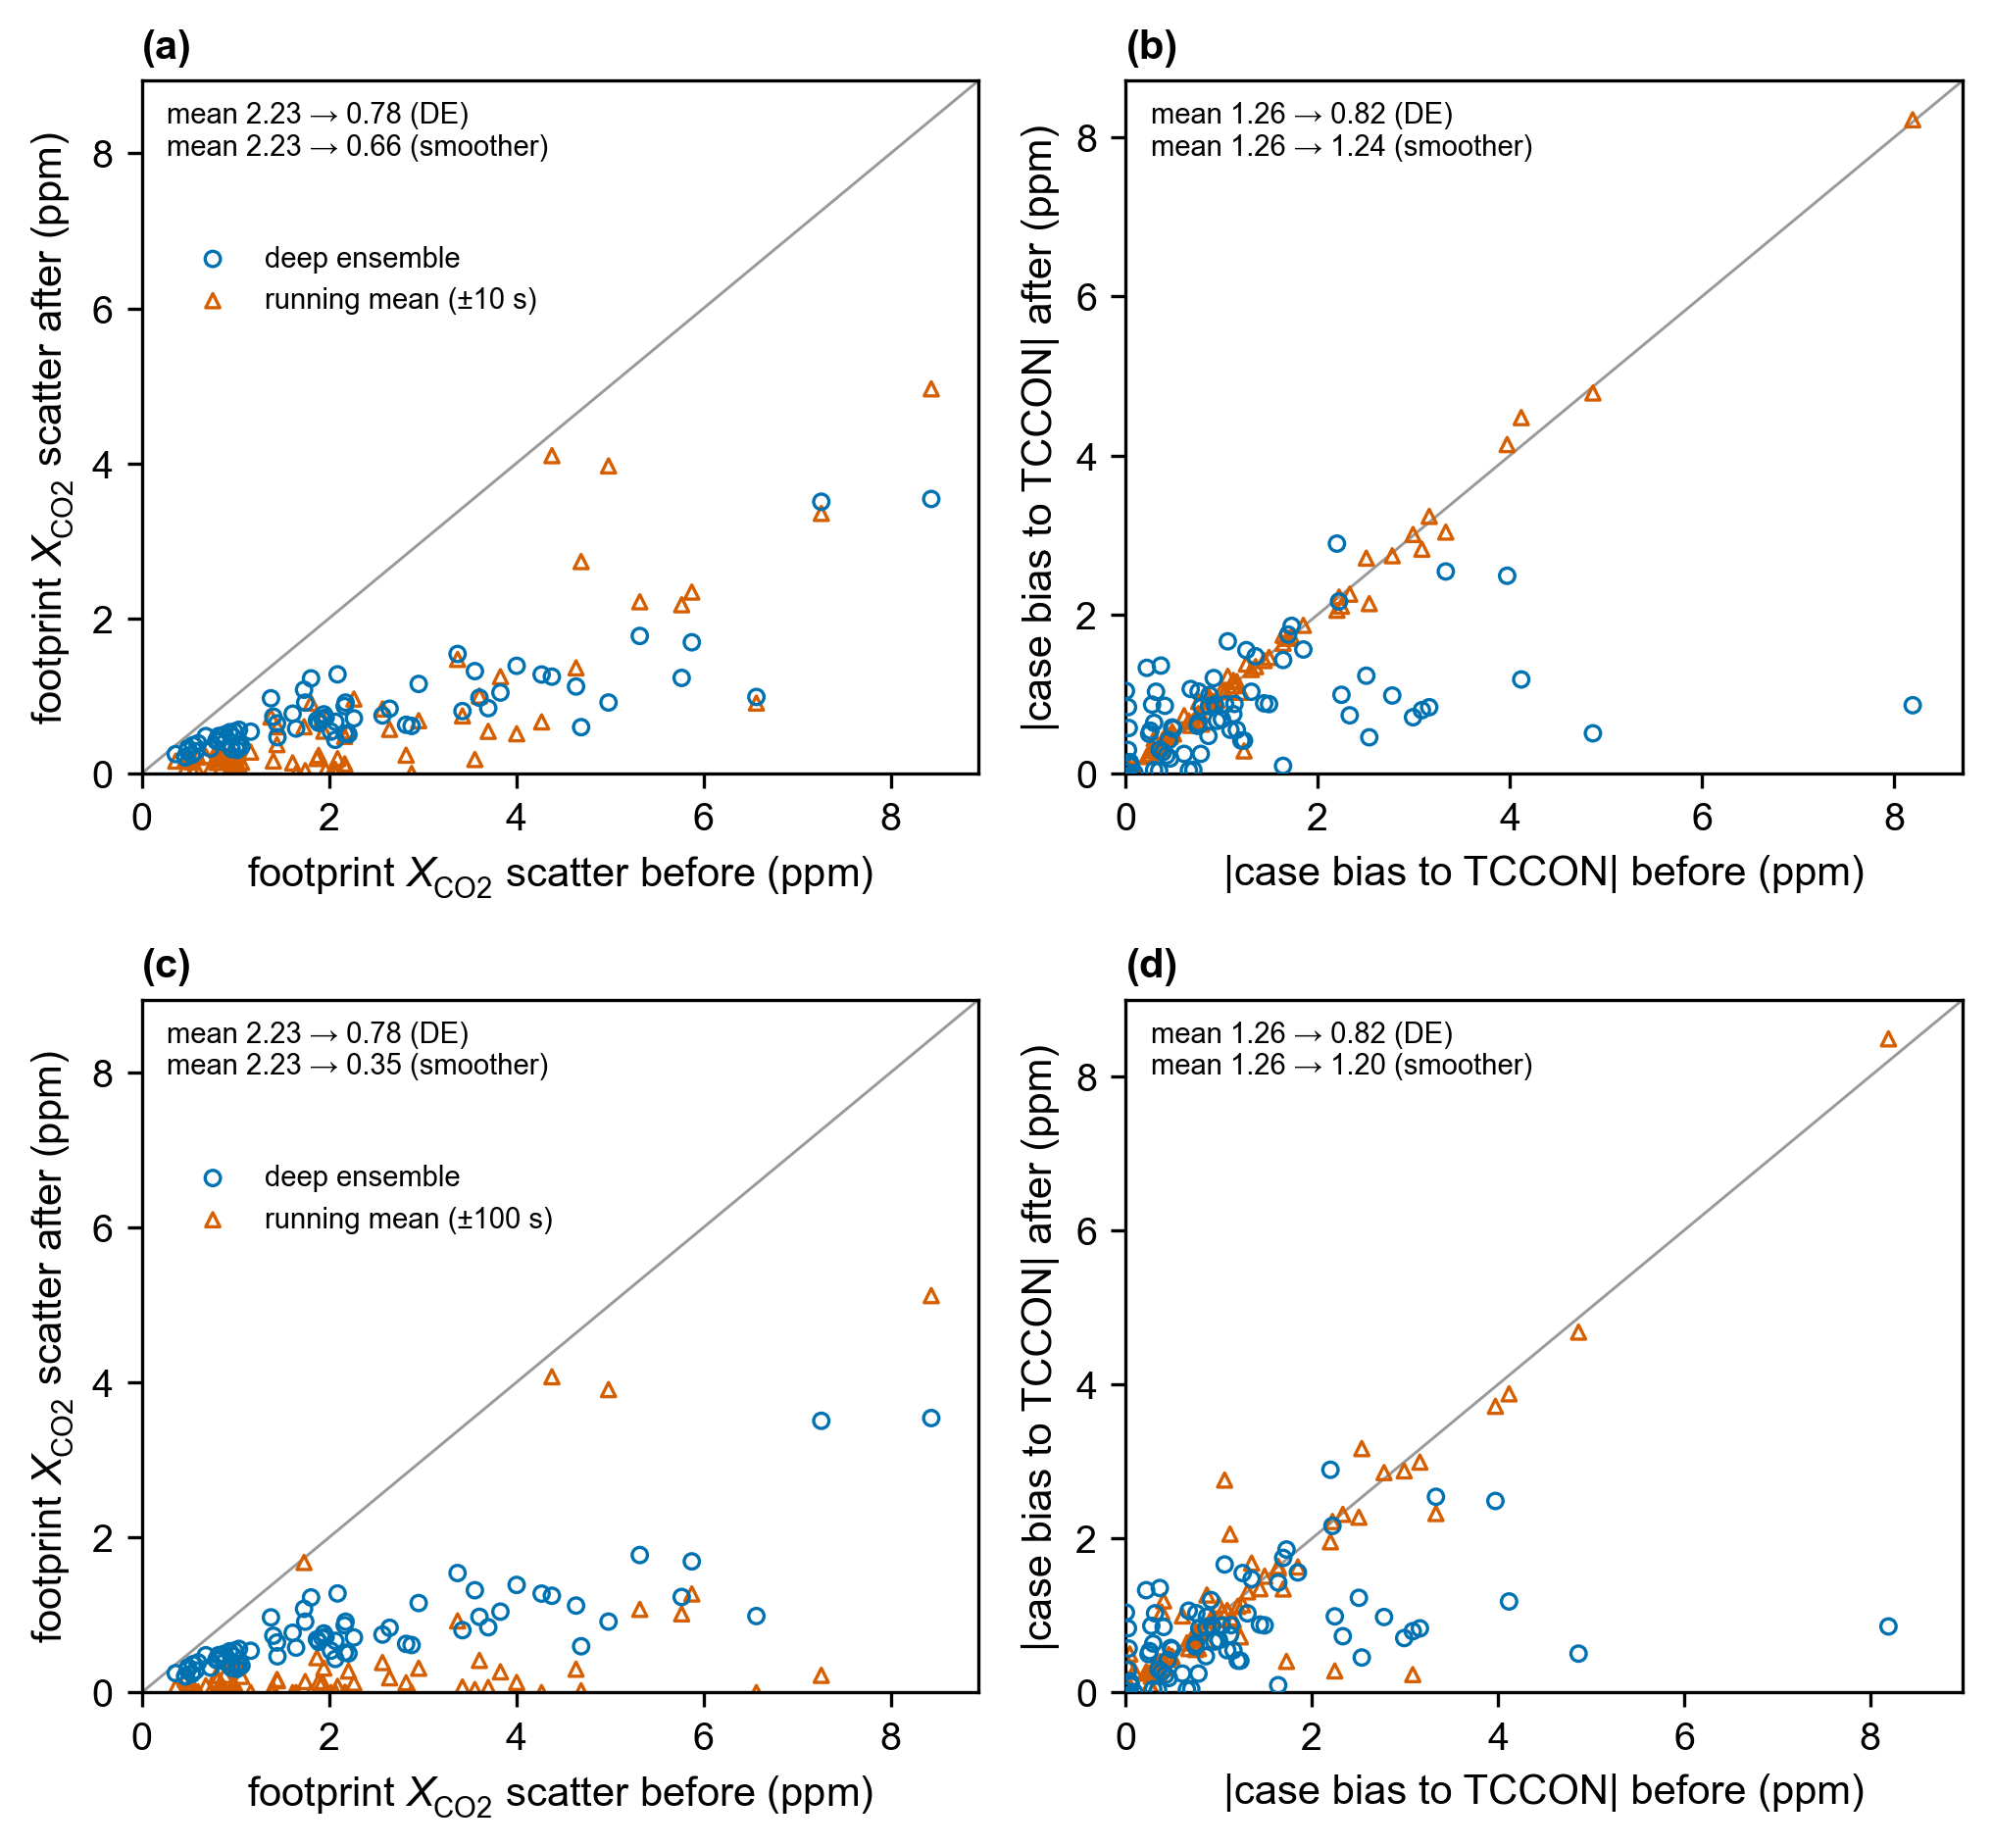
\includegraphics[width=0.8\textwidth]{figures/figE1_smoother_windows.png}
\caption{Feature-free smoother null: footprint-scatter collapse and TCCON station-day bias for orbit-local running-mean smoothers of half-width $\pm$10, $\pm$30, and $\pm$100 s beside the deep ensemble, under identical footprints, guards, and TCCON chain (windows not shown in main-text Fig.~\ref{fig:smoother_null}).}
\label{app-fig:smoother_null_full}
\end{figure}



\subsection{Negative controls}
\label{app:neg-control}



\begin{figure}[t]
\centering
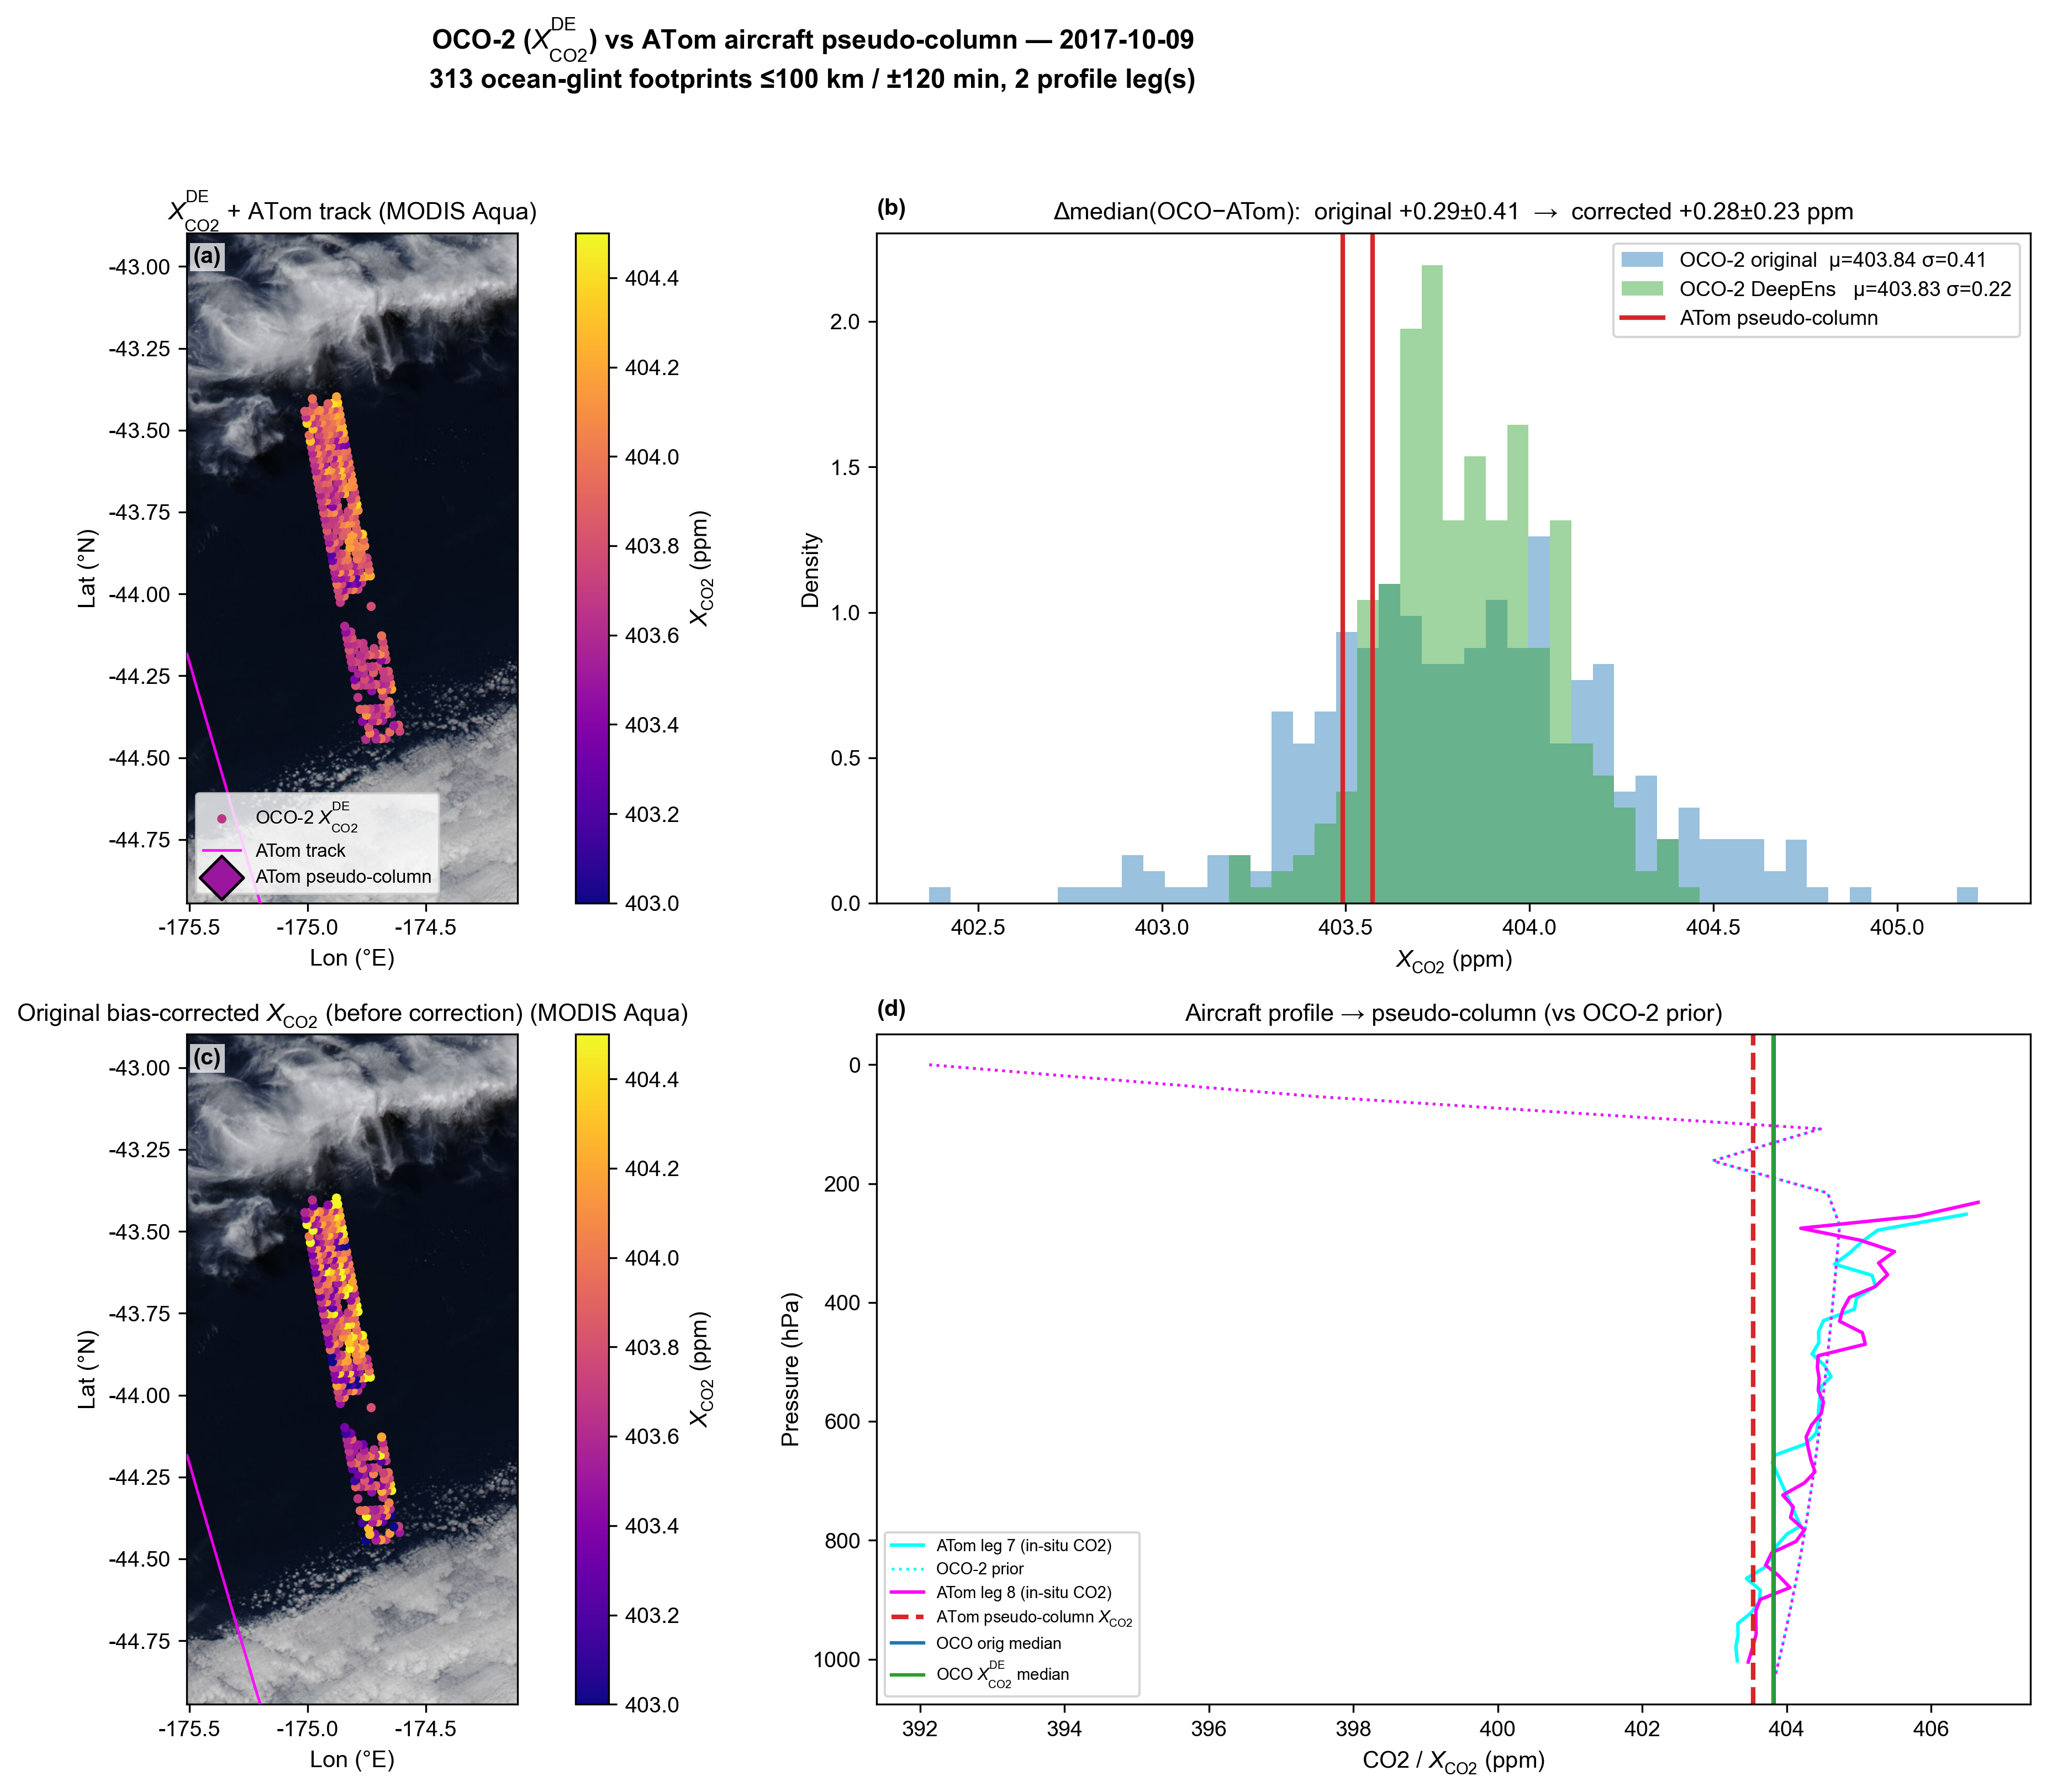
\includegraphics[width=0.8\textwidth]{figures/figE2_atom_farcloud_control.png}
\caption{ATom far-cloud negative control, 9 October 2017 (313 ocean-glint footprints within 100 km / ±120 min of two profile legs; median nearest-cloud distance 18 km): corrected and original \xco maps over the coincident MODIS Aqua true-colour scene (local day 8 October 2017 — the overpass crosses the antimeridian, where the imagery date is the local day) with the flight track, footprint distributions against the ATom pseudo-column, and the aircraft profiles with the OCO-2 prior.}
\label{app-fig:atom_far_cld}
\end{figure}


\begin{figure}[t]
\centering
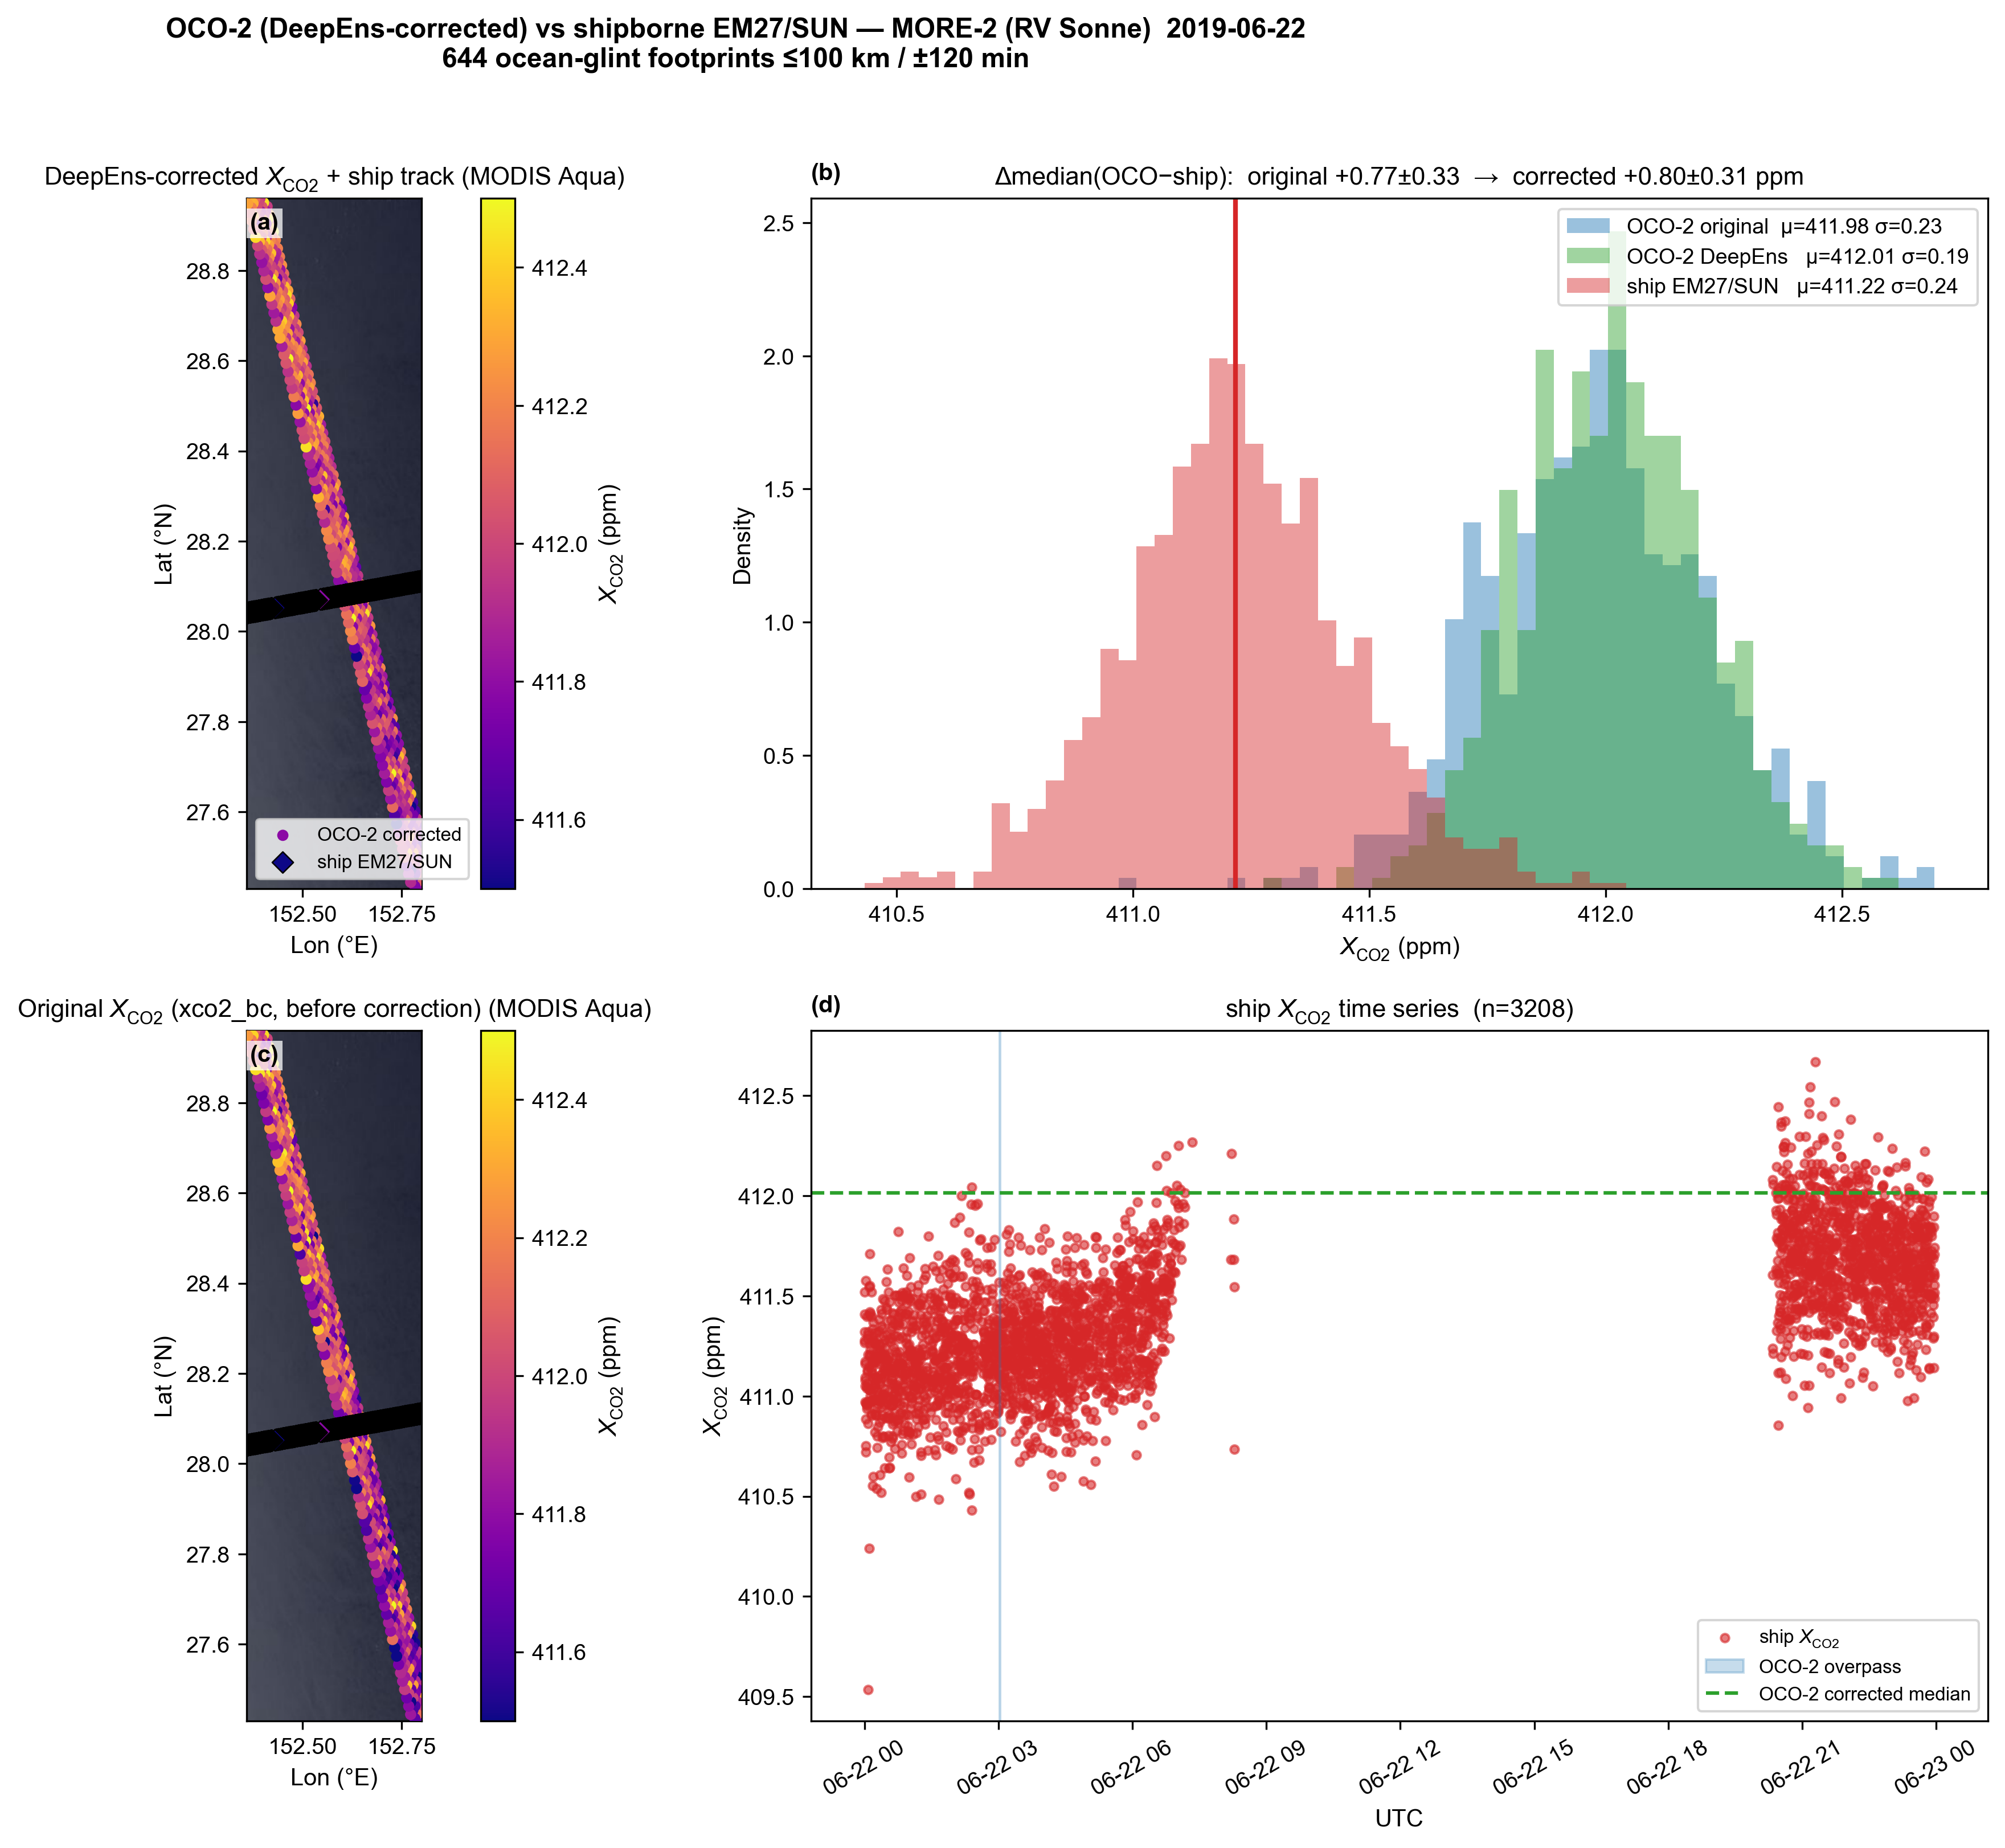
\includegraphics[width=0.8\textwidth]{figures/figE3_ship_clearday_control.png}
\caption{Shipborne clear-day negative control, 22 June 2019 (R/V Sonne EM27/SUN; 1 of 460 footprints within 10 km of cloud): same construction as Fig. E2 against the shipborne column, with the \xcoship time series around the overpass.}
\label{app-fig:ship_far_cld}
\end{figure}





\subsection{Failure cases analysis}
\label{app:tccon-failure}


\FloatBarrier